\chapter{Literature Review}
\section{Review method and evidence boundary}

This review is purposive and problem-led, selecting literature needed to justify artefact design,
evaluation and governance decisions. The local corpus documents source motivation, composition,
collection and processing, because useful documentation requires reflective context rather than
automated form completion \citep{gebru2021datasheets}. Reproducible reporting similarly depends on
explicit hypotheses, data, code, metrics and procedures \citep{pineau2021reproducibility}. The admitted
local corpus was checked and frozen on 27 August 2026; this dated state is not a systematic or PRISMA
review, meta-analysis, formal risk-of-bias assessment or exhaustive search.

Admission requires a stable local full-text file bound to a manifest row, checksum and bibliography
key. Each substantive claim is then checked against an exact page or passage. Visible references and
automatic citation metrics cannot establish correct or complete support by themselves
\citep{gao2023alce}; attribution also differs from answer correctness because a cited source may
itself be wrong \citep{gao2023rarr}. Search snippets, inaccessible pages and unsupported model
statements are excluded. Retained files, metadata and reporting details make the admission decision
reproducible \citep{pineau2021reproducibility}, while demonstrating internal traceability rather than
source truth.

Sources are tiered: peer-reviewed empirical studies, preprints, official guidance and official
technical documentation are not treated as interchangeable. Their stated unknowns, errors, risks and
non-applicable fields remain visible \citep{gebru2021datasheets}. Reproducibility means rerunning the
same analysis; it differs from independent replication, robustness and external validity
\citep{pineau2021reproducibility}. Methodological leakage, unavailable artefacts, incomplete reporting
and metric choices can still undermine machine-learning claims \citep{kapoor2023leakage}.
Accordingly, the synthesis supports this artefact's design rationale without estimating a pooled
effect, proving deployment performance across other organisations or operating contexts, or
introducing results from later chapters.

\clearpage
\begin{table}[p]
  \centering
  \caption{Review and local source-admission protocol}
  \label{tab:review-source-admission}
  \footnotesize
  \setlength{\tabcolsep}{3pt}
  \renewcommand{\arraystretch}{1.18}
  \hyphenpenalty=4000
  \exhyphenpenalty=4000
  \begin{tabularx}{\textwidth}{@{}P{0.17\textwidth}Y P{0.25\textwidth}P{0.24\textwidth}@{}}
    \toprule
    \rowcolor{WMGBlue!10}
    \textbf{Stage} &
    \textbf{Decision and action} &
    \textbf{Required local record} &
    \textbf{Reject or hold} \\
    \midrule
    \textbf{1. Problem-led discovery} &
    Search from the reporting problem, research questions and explicit evidence gaps; classify each candidate by intended source role. &
    Candidate title, origin and proposed use. Discovery alone does not admit a source. &
    Off-scope, duplicate or snippet-only candidates remain unadmitted. \\
    \addlinespace
    \rowcolor{DraftPale}
    \textbf{2. Stable local full text} &
    Obtain a complete, readable local PDF or an immutable permitted capture before claim use. &
    Stable local path plus origin and capture details where applicable. &
    Inaccessible, partial, snippet-only or no-stable-capture sources are held or rejected. \\
    \addlinespace
    \textbf{3. Manifest, checksum and bibliography binding} &
    Bind one citation key to bibliographic metadata, origin, local path, page count and SHA-256. &
    Manifest, checksum and bibliography agree; web-capture records agree when used. &
    Missing or duplicate key, absent row/hash, path reuse or any metadata/hash mismatch blocks admission. \\
    \addlinespace
    \rowcolor{DraftPale}
    \textbf{4. Page-level claim verification} &
    Inspect the local full text for the exact claim scope and record the supporting page locator. &
    Claim-ledger or section-evidence entry with source role, pages and verification state. &
    Unsupported, mis-scoped or unlocatable claims are rejected; citation presence does not prove truth. \\
    \addlinespace
    \textbf{5. Contradiction and limitation retention} &
    Preserve conflicts, unknowns, source hierarchy, reconstruction limits and non-applicable fields in synthesis. &
    Limitation and contradiction notes remain attached to the claim and source role. &
    Suppressed conflict, omitted caveat, source-tier equivalence or overclaim is held for repair. \\
    \addlinespace
    \rowcolor{DraftPale}
    \textbf{6. Strict freeze validation} &
    Run the strict local validator, then freeze the cited files and their bindings for the section. &
    Readable files; matching manifest, checksums, bibliography and capture records; resolvable claim locators. &
    Missing/unreadable file, unresolved citation, mutable-only reference or any binding mismatch blocks freeze. \\
    \bottomrule
  \end{tabularx}
  \vspace{3pt}

  \parbox{\textwidth}{\scriptsize
    \textit{Method status:} Purposive, problem-led, non-systematic and non-exhaustive; not PRISMA.\\
    \textit{Source note:} Author synthesis of frozen local source-admission contracts, not results. Local storage, hashing and citation presence establish traceability controls, not source truth.
  }
\end{table}
\clearpage


\section{Early-stage finance, portfolio reporting, and public company intelligence}

Early-stage finance involves information asymmetry: founders know more about ventures than dispersed
investors, while platforms shape what is disclosed and observed. Cross-country crowdfunding evidence
shows that amounts raised and investor participation vary with pitch, sector, region, country and
platform; its analysed sample covers successful pitches rather than all attempts
\citep{estrin2024digital}. A Crowdcube study likewise associates successive rounds with investor
responses and funding outcomes within one platform-specific campaign sample
\citep{wasti2024successive}. Such observations can organise portfolio context, but neither investor
count nor a completed round is a universal or causal label of firm quality or future performance.

Portfolio intelligence should represent finance and state support as attributed events with dates and
sources. In the Crowdcube setting, a prior successful round may be interpreted as a signal, but the
relationship remains conditional on campaign and platform characteristics
\citep{wasti2024successive}. Linked UK public-support research observes later differences among
participating firms, while retaining selection explanations and declining to claim causality
\citep{mondal2025state}. Reconstructing the UK funding lifecycle also requires joining opportunities,
applications, decisions, projects, organisations and outcomes without common identifiers; coverage
and conservative links remain incomplete \citep{thorne2026funding}. A round, grant or award can
support a dated statement, not proof of future success or a complete funding history.

Public company intelligence needs a legal anchor before these events can be joined. A Companies House
number identifies a registered entity, and incorporation data provide timely, broad visibility of
company creation; however, incorporation is not economic activity, and the register includes dormant
firms while excluding some unincorporated activity \citep{galanakis2026chrt}. Whole-register analysis
is tied to a dated snapshot, corporate forms and filing definitions, with recent records affected by
filing lag \citep{hardman2023small}. Register usefulness depends on intended use and on content quality,
accessibility and interpretation, not openness alone \citep{krasikov2020ready}. Registry status and
filings are therefore evidence about a legal record, not a complete operational or financial profile.

The synthesis sets a reporting boundary, not an investment model. Each admissible statement should
identify the event, legal entity, source, observation or availability date, exact locator and supported
content; gaps, linkage uncertainty and conflicts should remain visible. This matters because
crowdfunding evidence is sample- and platform-dependent \citep{estrin2024digital}, while differences
associated with public support can reflect selection rather than causal impact
\citep{mondal2025state}. Financial communications can influence investment decisions and should
present relevant benefits and risks clearly and fairly \citep{fca2024promotions}. Portfolio reporting
should therefore not generate buy/sell advice, speculative valuation, causal performance attribution
or a universal company-quality score. These limits define evidence-calibrated synthesis, not artefact
results.

\clearpage
\begin{table}[p]
  \centering
  \caption{Signal-to-inference boundary for early-stage company intelligence}
  \label{tab:signal-inference-boundary}
  \footnotesize
  \setlength{\tabcolsep}{2.2pt}
  \renewcommand{\arraystretch}{1.16}
  \begin{tabularx}{\textwidth}{@{}P{0.152\textwidth}P{0.188\textwidth}P{0.22\textwidth}Y>{\RaggedRight\arraybackslash\scriptsize}p{0.15\textwidth}@{}}
    \toprule
    \rowcolor{WMGBlue!10}
    \textbf{Evidence class} &
    \textbf{Observable / source-bound fact} &
    \textbf{Admissible report statement} &
    \textbf{Unsupported inference} &
    {\rmfamily\footnotesize\textbf{Key local literature}} \\
    \midrule
    \textbf{Crowdfunding}\par\textbf{/ funding round} &
    Attributed platform or publisher record of a campaign or round, with its date, disclosed stage or amount, and source scope where stated. &
    ``The named source records this entity's campaign or funding event on the stated date.'' Include the exact locator and qualify platform or sample scope. &
    Proof of firm quality, universal investor preference, causal impact, future performance or investment merit. &
    estrin2024\allowbreak digital\par wasti2024\allowbreak successive \\
    \addlinespace
    \rowcolor{DraftPale}
    \textbf{Public grant or state-support record} &
    Named programme, recipient, award or support event, date, publisher and explicit amount/currency where available. &
    ``The publisher records the named award or support event for this legal entity.'' State the date, locator, cutoff and any amount-coverage limit. &
    That support caused innovation or growth; that the recipient is superior; complete support history or measured impact. &
    mondal2025\allowbreak state\par thorne2026\allowbreak funding\par fca2024\allowbreak promotions \\
    \addlinespace
    \textbf{Companies House identity / filing event} &
    Exact company number plus a legal name, status, incorporation or filing event from a dated register snapshot. &
    ``At the stated cutoff, the register records this legal fact or filing for company number X.'' Retain filing period and register scope. &
    Incorporation as active trading; complete operations, ownership or financial health; private funding, valuation or current state beyond the cutoff. &
    galanakis2026\allowbreak chrt\par hardman2023\allowbreak small\par krasikov2020\allowbreak ready \\
    \addlinespace
    \rowcolor{DraftPale}
    \textbf{Reconstructed}\par\textbf{funding-lifecycle link} &
    Conservatively linked events whose component sources, identifiers, dates, linkage rule and unmatched gaps remain visible. &
    ``These attributed records form a partial reconstructed timeline for the same legal entity under the stated linkage rule.'' &
    Exhaustive funding history; absence as proof of no event; a causal pathway, universal lifecycle or forecast of success. &
    thorne2026\allowbreak funding\par mondal2025\allowbreak state \\
    \bottomrule
  \end{tabularx}
  \vspace{3pt}

  \parbox{\textwidth}{\scriptsize
    \textit{Interpretation:} Author synthesis; non-empirical and not a scoring, ranking, valuation, recommendation or causal model.\\
    \textit{Source note:} Locally admitted keys estrin2024digital, wasti2024successive, mondal2025state, thorne2026funding, galanakis2026chrt, hardman2023small, krasikov2020ready and fca2024promotions; claim scope follows ledger rows 2.2-P1--2.2-P4.
  }
\end{table}
\clearpage


\section{Data quality, entity identity, missingness, and time}

Data quality is fitness for a stated task, not one context-free dataset property. Dimensions such as
accuracy, reliability, timeliness, completeness and consistency need validation rules attached to the
relevant data object \citep{nikiforova2020quality}. Corporate-register evidence reinforces this
use-case view: accessibility and open availability do not ensure that content is complete,
interpretable or suitable for a particular enterprise purpose \citep{krasikov2020ready}. Portfolio
reporting should therefore state each field's intended use and test the dimensions material to it. A
generic aggregate score could hide a failure important to one reporting purpose but immaterial to
another. It cannot establish fitness across purposes.

Entity resolution is similarly source-scoped. An exact company number from the authoritative register
is the legal-identity anchor; a name is only a candidate-generating label. Funding sources without
shared identifiers require conservative exact or fuzzy linkage, yet coverage and matching errors
remain \citep{thorne2026funding}. Cross-register work also required normalisation, fuzzy comparison and
manual matching when entity and country labels conflicted \citep{surak2026gateways}. Companies House
identifies incorporated legal entities, not economic activity itself \citep{galanakis2026chrt}.
Consequently, uncertain matches must remain unresolved or enter a conflict/review state pending named
review rather than silently merging records with similar names.

Missingness must preserve meaning rather than become a default number. Documentation should record
what is absent, why and what remains unknown \citep{gebru2021datasheets}. Financial-table structure
distinguishes populated cells, empty cells, positions and semantic roles; an empty cell is not
automatically zero \citep{bradley2024synfintabs}. Completeness and validity are separate dimensions
requiring task-specific checks \citep{nikiforova2020quality}. This project therefore distinguishes
blank, zero, explicit none, not applicable, not reported, not found publicly, invalid and observed.
Not found publicly does not mean absent. This exact taxonomy is the artefact's design choice, not a
universal standard derived from the literature.

Time also requires separate fields. The value period records when an event occurred; publication or
effective time records when it became available; retrieval time records collection; and the reporting
cutoff limits eligible evidence. Dated register snapshots and filing lag show why recent facts may be
unavailable earlier at that cutoff \citep{hardman2023small}, while incorporation and later economic
activity follow different clocks \citep{galanakis2026chrt}. Using information published after a
historical cutoff creates temporal leakage and can inflate evaluation \citep{kapoor2023leakage}. A
correction must create a new version with its own timestamp, never retrospectively support an earlier
report.

Together, these distinctions form an evaluable evidence contract. Identity, missing state, value
period, availability time, source, locator and version must be typed; invalid, conflicting and held
states remain visible; and each rule is testable before synthesis or comparison. Checks should be tied
to the user task and data object \citep{nikiforova2020quality}. Documentation should expose unknowns,
errors, dependencies and correction practices \citep{gebru2021datasheets}, while evaluation must guard
against leakage and under-specified comparisons \citep{kapoor2023leakage}. This contract gives a
literature-based rationale for later methodology; it neither claims completed implementation nor
reports empirical results.

\clearpage
\begin{table}[p]
  \centering
  \footnotesize
  \setlength{\tabcolsep}{2.2pt}
  \renewcommand{\arraystretch}{1.16}
  \begin{tabularx}{\textwidth}{@{}P{0.15\textwidth}P{0.24\textwidth}P{0.19\textwidth}Y>{\RaggedRight\arraybackslash\scriptsize}p{0.14\textwidth}@{}}
    \toprule
    \textbf{Data control} &
    \textbf{Required distinction} &
    \textbf{Unsafe combination} &
    \textbf{Effect on reporting or evaluation} &
    {\footnotesize\textbf{Key local literature}} \\
    \midrule
    \textbf{Legal identity} &
    Keep an exact source-scoped legal identifier separate from names, domains and aliases; hold unresolved candidates or conflicts. &
    Name-only or fuzzy auto-merge; treating incorporation as economic activity. &
    Evidence can attach to the wrong company, contaminating reports and identity accuracy or coverage measures. &
    thorne2026\allowbreak funding\par surak2026\allowbreak gateways\par galanakis2026\allowbreak chrt \\
    \addlinespace
    \textbf{Observed value / missing state} &
    Separate a value from the reason it is missing. The project distinguishes observed, zero, blank, explicit none, not applicable, not reported, not found publicly and invalid. &
    Treating null, blank, no record, invalid and zero as equivalent. &
    False totals or absence claims follow; blank-zero and missing-state evaluation becomes invalid. &
    gebru2021\allowbreak datasheets\par bradley2024\allowbreak synfintabs\par nikiforova2020\allowbreak quality \\
    \addlinespace
    \textbf{Publication / effective / retrieval / cutoff time} &
    Retain value period, publication or effective availability, retrieval time and reporting cutoff separately. &
    One timestamp; retrieval treated as publication; later evidence used at an earlier cutoff. &
    Leakage across time, old or future claims and an unfair historical evaluation. Evidence from the wrong date must be held. &
    hardman2023\allowbreak small\par galanakis2026\allowbreak chrt\par kapoor2023\allowbreak leakage \\
    \addlinespace
    \textbf{Correction / version / snapshot} &
    Keep write-once source bytes and checksum, data meaning, schema and source versions, and each later correction as a new dated version. &
    Overwrite the earlier snapshot or silently backfill a correction into a past report. &
    Claims and calculation totals cannot be repeated. Historical comparisons and links to approval become invalid. &
    gebru2021\allowbreak datasheets\par hardman2023\allowbreak small\par kapoor2023\allowbreak leakage \\
    \addlinespace
    \textbf{Use-case data quality} &
    Assess explicit dimensions and executable rules against the named data object and reporting task. &
    One context-free quality score, or assuming open availability means fitness. &
    The cause of failure becomes unclear, eligibility rules are applied wrongly and results across tasks cannot be compared fairly. &
    nikiforova2020\allowbreak quality\par krasikov2020\allowbreak ready \\
    \bottomrule
  \end{tabularx}

  \caption{Data meanings that must remain separate}
  \label{tab:data-semantics-matrix}
  \vspace{3pt}

  \parbox{\textwidth}{\scriptsize
    \textit{Meaning:} Developed by the author and not a result. The exact list of missing states is a project choice, not a published or universal standard.\\
    \textit{Source note:} The local sources are thorne2026funding, surak2026gateways, galanakis2026chrt, gebru2021datasheets, bradley2024synfintabs, nikiforova2020quality, hardman2023small, kapoor2023leakage and krasikov2020ready. Supporting pages are in claim-ledger rows 2.3-P1--2.3-P5.
  }
\end{table}
\clearpage


\section{Provenance, source admission, contradiction, and auditable synthesis}

Provenance is a chain of custody for a statement, not a certificate of truth. Documentation should
record data motivation, composition, processing, known gaps and errors, external dependencies,
distribution, maintenance and corrections \citep{gebru2021datasheets}. Reproducible reporting
requires data, code, procedures and metrics sufficient to repeat an analytical path
without extending claims beyond its evidence \citep{pineau2021reproducibility}. For portfolio
synthesis, provenance should bind each statement to its source record, captured artefact, exact
locator, transformations and admission, verification and approval decisions. This supports internal
traceability and repeatability while leaving source authority, factual truth and completeness for
separate assessment.

Source admission and claim fit are separate gates. Admission tests a source against policy
on accessibility, type, use rights, date and stable capture. Claim fit asks whether an exact passage
supports the bounded statement. Citation entailment and completeness differ from answer
correctness; visible references may still be irrelevant or partial \citep{gao2023alce}. Retrieved
material may be ignored, contradicted or faithfully attributed even when its source is wrong
\citep{gao2023rarr}. Reproducibility depends on reporting these decisions and artefacts
\citep{pineau2021reproducibility}. Search snippets, bare URLs and fluent summaries therefore pass
neither gate alone.

An admitted artefact should be captured immutably where permitted and technically possible.
Its record should retain checksum, retrieval time, exact page or passage locator and source version; a
correction creates a new version rather than overwriting the earlier state. Dataset documentation
supports recording external resources, distribution, updates, errata and older versions
\citep{gebru2021datasheets}, while reproducibility requires sufficient artefacts and procedures
\citep{pineau2021reproducibility}. Model-card work similarly separates version, intended use,
evaluation procedure, limitations and caveats \citep{mitchell2019modelcards}. These record fields are
project design choices; immutable capture is not universally permitted.

Contradiction is an evidence state, not noise to remove. Hallucination research distinguishes factual
contradiction, unverifiable content and overclaiming, and links reliable output to uncertainty and
verification against trusted knowledge \citep{huang2023hallucination}. Attribution does not resolve
disagreement when evidence conflicts with generated text or its source is wrong
\citep{gao2023rarr}; a citation marker also cannot collapse correctness, entailment and completeness
into one judgement \citep{gao2023alce}. Inconsistent but supported claims should remain a conflict
set, while unverifiable material is held. Resolution requires a declared rule or named review, not
automatic preference for the majority, newest or most fluent version. The exact conflict taxonomy is
not claimed as universal.

Auditable synthesis records candidate discovery, admission, capture, typed claim, support check,
contradiction state, approval and export decisions. Rigorous measurement should document uncertainty,
benchmarks, evaluated conditions and independent-review limits \citep{nist2023airmf}. Independent
verification should assess support without rewriting the primary statement, because answer
correctness, citation correctness, citation completeness and attribution are distinct
\citep{gao2023alce,gao2023rarr}. Human-facing systems should communicate uncertainty and permit
correction or dismissal before consequential action \citep{amershi2019guidelines}. Only supported and
approved claims should proceed to export. This literature-based rationale does not
show that independent or human review improves outcomes, user benefit or deployment safety.

\begin{figure}[htbp]
  \centering
  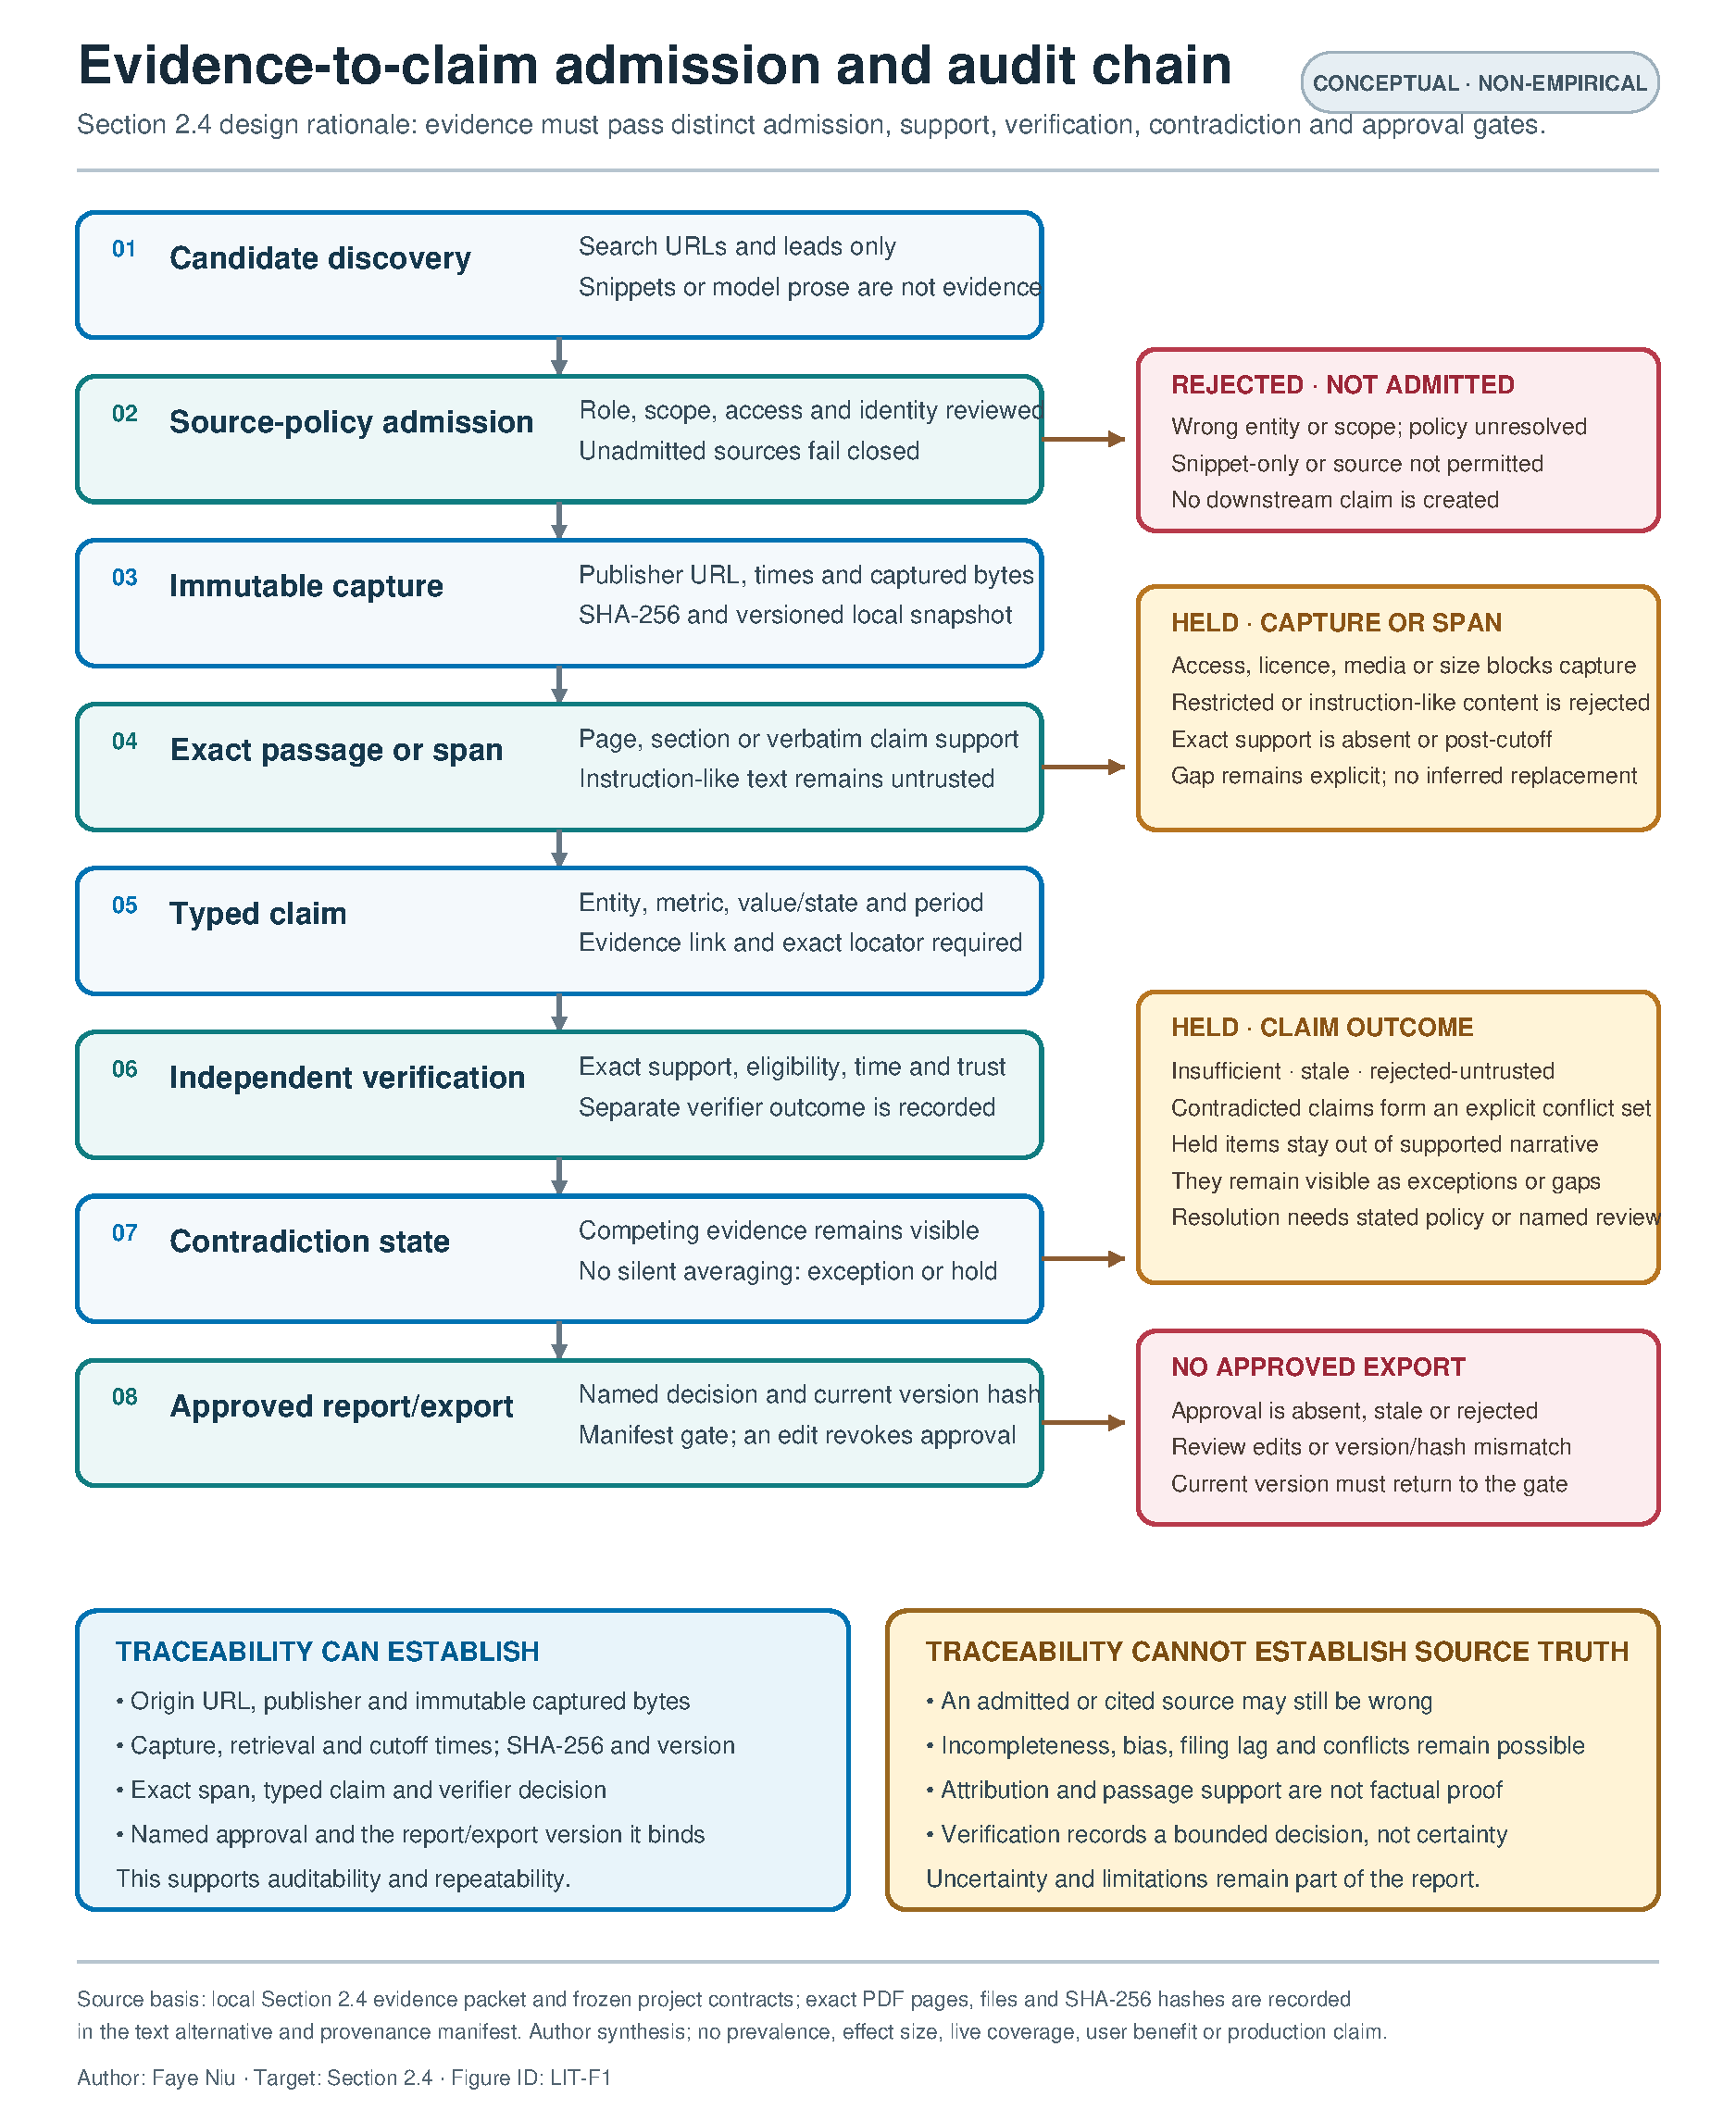
\includegraphics[width=0.82\textwidth,height=0.78\textheight,keepaspectratio]{exhibits/lit_f1_evidence_claim_admission_audit_chain.pdf}
  \caption{Evidence-to-claim admission and audit chain. Author synthesis of the cited literature and
  frozen project contracts; conceptual and non-empirical.}
  \label{fig:lit-evidence-claim-chain}
\end{figure}

\section{LLM-assisted discovery and grounded extraction}

Retrieval-augmented generation (RAG) separates indexing, retrieval and generation, but does not
guarantee evidence-grounded output. Nor does retrieved context establish source quality, completeness
or factual truth. Retrieval may omit relevant material, select irrelevant chunks or shape unsupported
answers \citep{gao2023ragsurvey}. External retrieval can reduce knowledge gaps while inaccurate
material still creates misleading output \citep{huang2023hallucination}; attribution also remains
separate from correctness \citep{gao2023rarr}. LLM assistance may therefore widen candidate
discovery, but retrieval, source admission, extraction and verification must remain separate gates.

The captured Responses API documentation describes model-managed \texttt{web\_search}, inline
citations and annotations, domain filters and a consulted-source list
\citep{openai2026websearch}. These features suit query planning and candidate inventory within
modular retrieval designs \citep{gao2023ragsurvey}. However, settings do not guarantee source or
citation counts, and visible citations can remain incomplete or unsupported \citep{gao2023alce}. The
documentation establishes capability on its capture date, not executed behaviour or performance;
returned URLs, snippets, annotations and model prose remain candidates pending admission.

Grounded extraction should be deterministic first for structured evidence. Admitted unstructured
public or synthetic evidence may instead use bounded, optional model-assisted extraction, but only to
propose a typed claim linked to an exact passage. Answer correctness, citation entailment and citation
completeness remain distinct \citep{gao2023alce}, while attribution does not establish correctness
when evidence disagrees \citep{gao2023rarr}. Both routes must converge on deterministic exact-span and
schema validation, normalisation and independent verification, reflecting separate relevance,
faithfulness, rejection and robustness checks \citep{gao2023ragsurvey}. Unsupported content is
rejected or held, never repaired from model memory; this ordering is the artefact's design choice.

Retrieved public content must remain untrusted data, not instruction authority. Indirect prompt
injection can embed adversarial instructions in searched material and manipulate summaries, queries,
sources or downstream actions \citep{greshake2023indirect}. RAG is also exposed to noisy,
contradictory and adversarial context \citep{gao2023ragsurvey}. Research controls should therefore fix
tool permissions, validate destinations, isolate extraction, bound redirects and requests, and fail
closed. Testing, uncertainty, independent review and safe failure are risk-management principles
\citep{nist2023airmf}; the literature justifies these controls but does not prove their effectiveness
here.

Coverage should be a recorded research budget, not a claim to have searched the web comprehensively.
Search context, token budgets, live-access controls, domain filters and source lists are configurable,
while search may be optional and source counts are not guaranteed \citep{openai2026websearch}.
Evaluation should separate correctness, citation support and completeness \citep{gao2023alce} from
relevance, faithfulness, rejection, integration and robustness \citep{gao2023ragsurvey}. A repeatable
protocol records queries, sources, cutoff time, token and cost bounds, then reports inaccessible,
missing, conflicting and unverified areas \citep{pineau2021reproducibility}; it cannot estimate
open-web recall.

\begin{figure}[htbp]
  \centering
  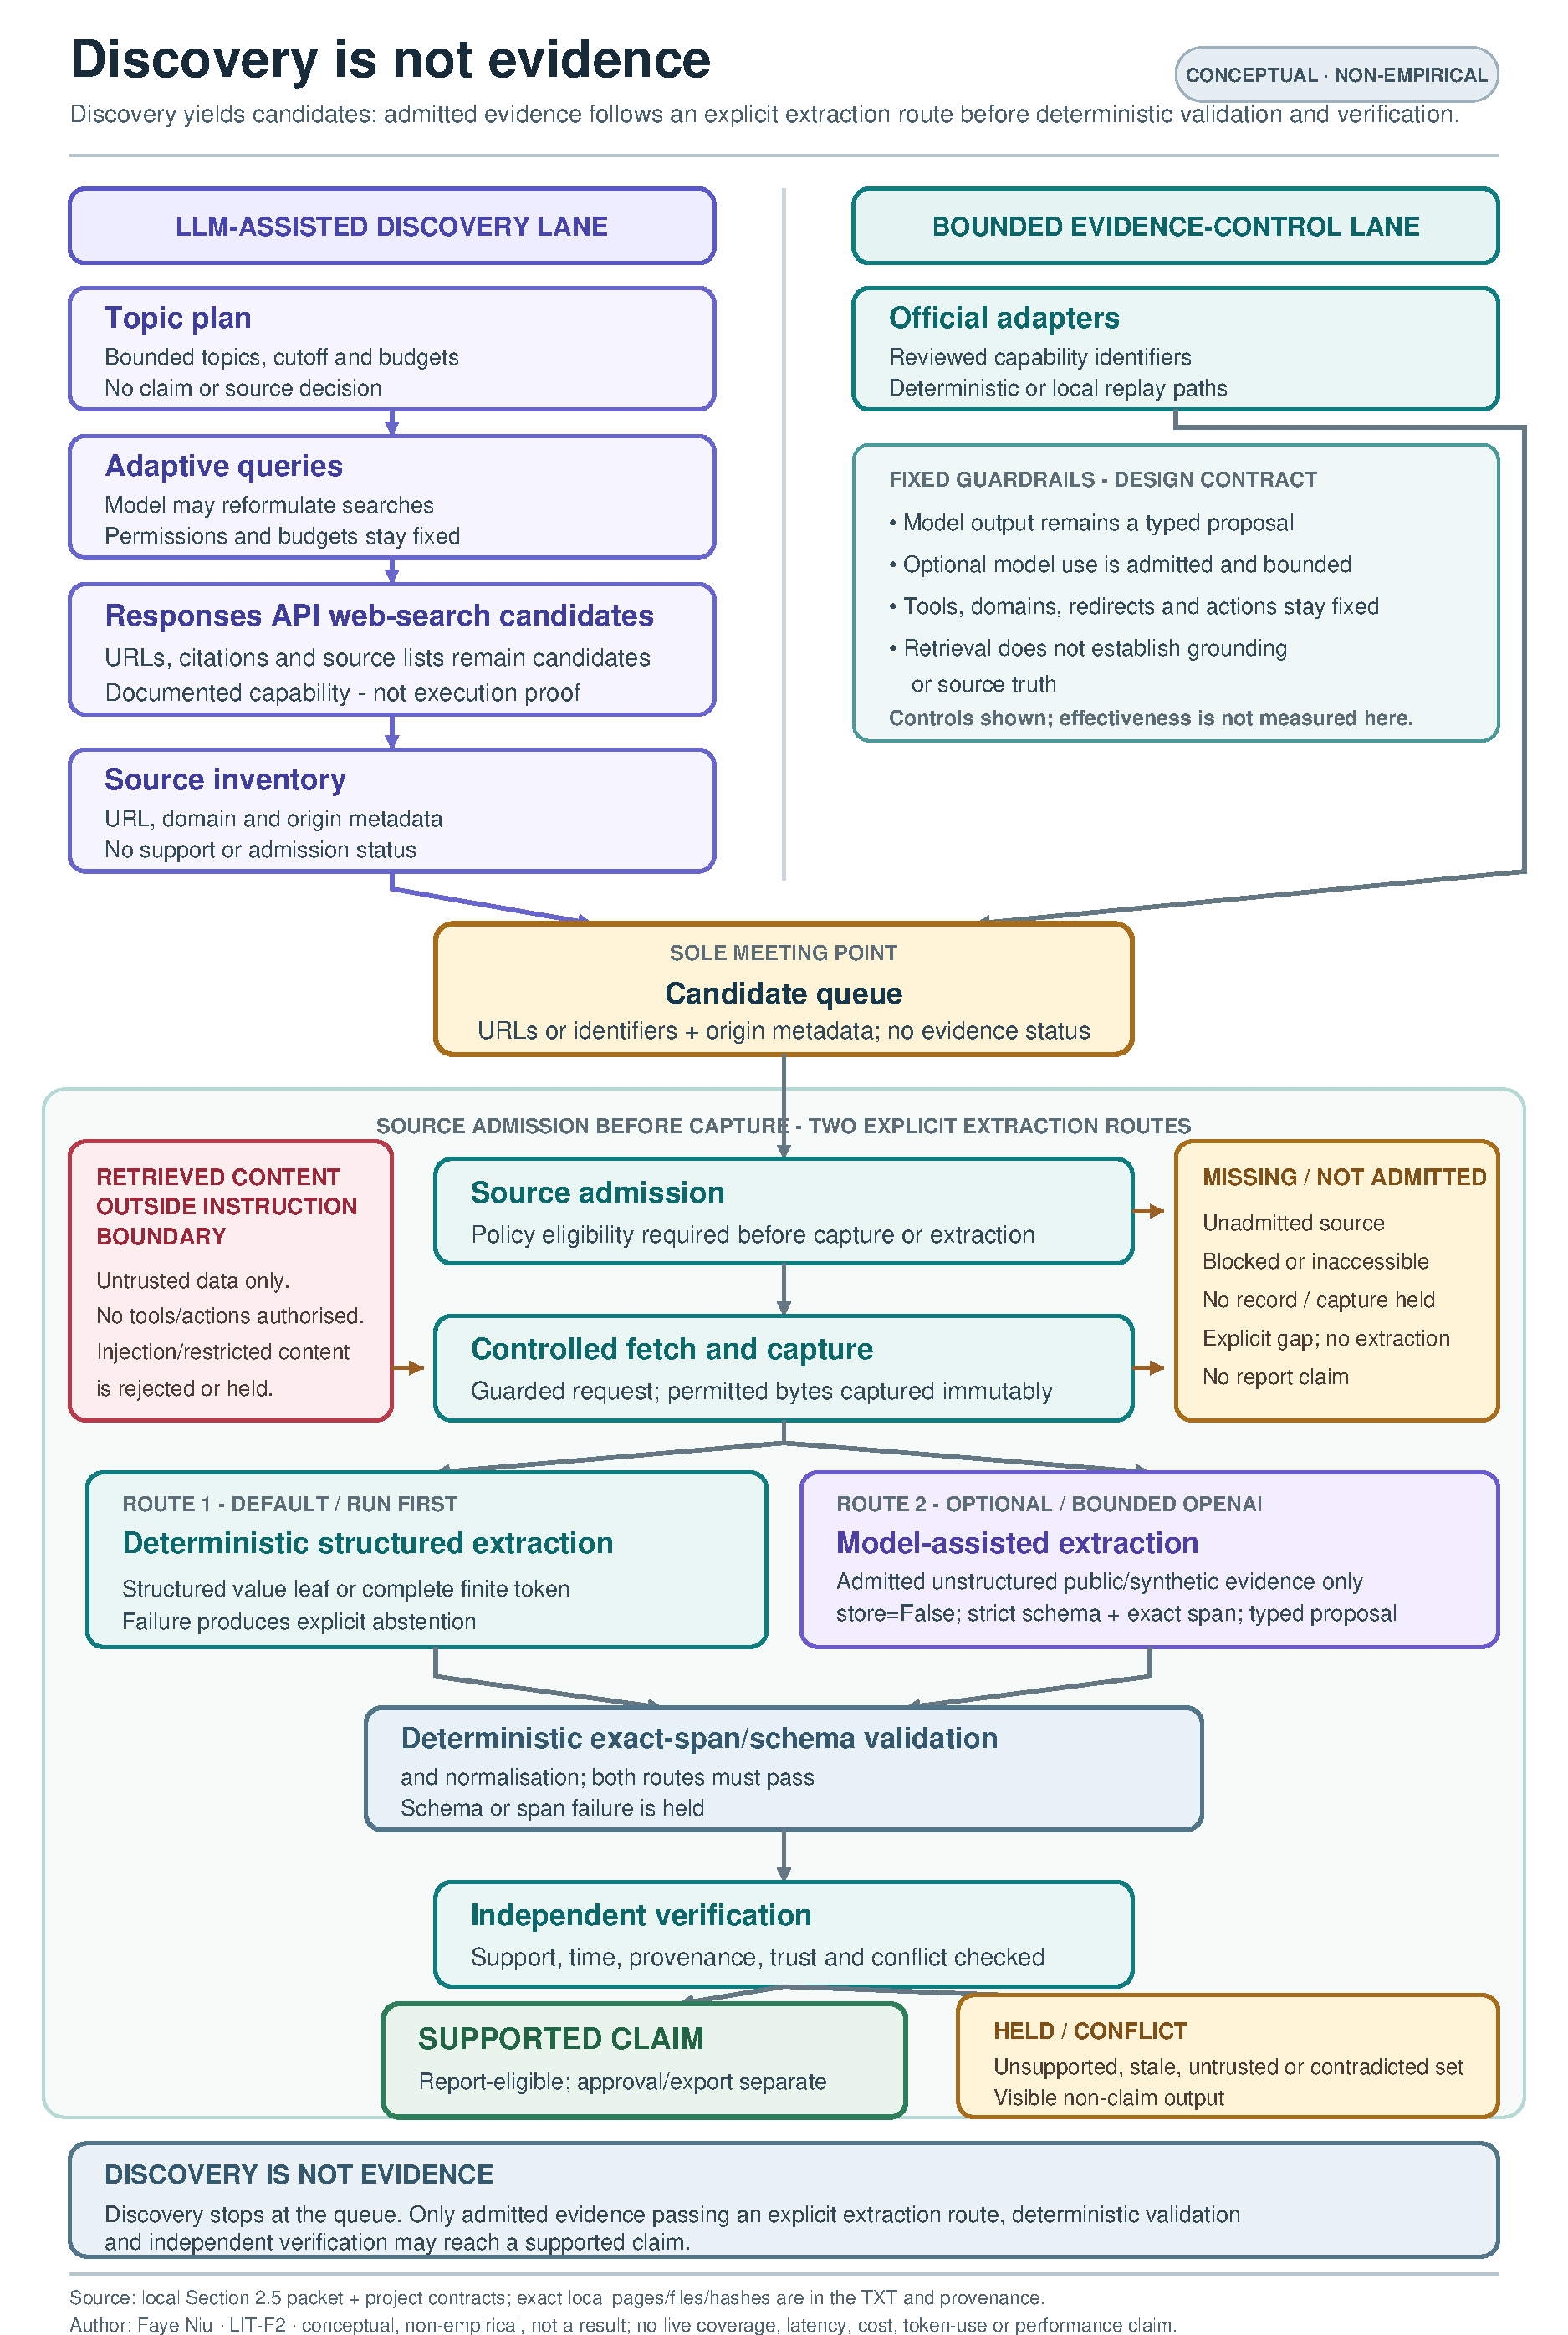
\includegraphics[width=0.82\textwidth,height=0.78\textheight,keepaspectratio]{exhibits/lit_f2_discovery_is_not_evidence.pdf}
  \caption{Discovery is not evidence. Author synthesis of the cited literature and frozen project
  contracts; conceptual and non-empirical.}
  \label{fig:lit-discovery-evidence-boundary}
\end{figure}
\clearpage

\section{Bounded multi-agent systems and human review}

A multi-agent workflow is a programmed decomposition, not evidence of collective intelligence.
Surveyed systems vary in environment interfaces, profiles, communication structures and message
content \citep{guo2024multiagent}, while AutoGen shows that developers configure roles,
capabilities, tools, human-input modes, control flow and termination \citep{wu2024autogen}.
Table~\ref{tab:lit-role-authority-matrix} makes explicit that each role needs a distinct
responsibility, typed input/output contract and observable failure boundary. A role label or conversation does not establish
competence, independence or benefit; design-science evaluation must test whether the resulting
artefact meets its stated objectives \citep{peffers2007dsrm}.

Orchestration should therefore be serial, budgeted and explicit. Communication topology determines
information flow, while hallucinated content can propagate and additional roles add coordination,
communication and resource costs \citep{guo2024multiagent}. Programmed control flow, tool rules,
human-input conditions and termination criteria are necessary to bound execution
\citep{wu2024autogen}. Typed handoffs, retry limits and stop reasons should remain visible. An
independent verifier records whether evidence supports a claim and may reject or hold it, but must
not rewrite the producer record. This separation permits evaluated conditions and uncertainty to be
documented \citep{nist2023airmf}; it does not imply that more roles are better.

Human review supplies decision authority, not additional evidence. Interfaces should expose the
claim, exact support, conflicts, uncertainty, limitations and content hash, then allow a named
reviewer to approve, reject or return the record for correction. Human--AI guidance supports
invocation, dismissal, correction and global controls \citep{amershi2019guidelines}, but it is not
outcome evidence. Explanations alone may not prevent overreliance; one controlled task found
trade-offs in performance, usability and participant effects \citep{bucinca2021forcing}. Oversight
must therefore be defined for the context and risk tolerance \citep{nist2023airmf}, without claiming
improved accuracy, trust or utility before an authorised study.

Evaluation must treat failures and limits as first-class records. Multi-agent systems face
hallucination propagation, coordination, scalability and incomplete-benchmark problems
\citep{guo2024multiagent}; AutoGen's configurable roles and application-specific pilots do not
establish universal superiority \citep{wu2024autogen}. Logs should retain role, task and attempt
identifiers, inputs, outputs, hashes, duration, tokens, errors, stop reasons, cancellation and recovery
state. Frozen cases should test each role and the full workflow, including disagreement and safe
failure, with procedures and metrics reported for repeatability
\citep{nist2023airmf,pineau2021reproducibility}. Agent count, message count and conversation
completion are not measures of task success.

\clearpage
\begin{table}[p]
  \centering
  \caption{Role-and-authority matrix for bounded multi-agent reporting}
  \label{tab:lit-role-authority-matrix}
  \footnotesize
  \setlength{\tabcolsep}{2.1pt}
  \renewcommand{\arraystretch}{1.16}
  \hyphenpenalty=3500
  \exhyphenpenalty=3500
  \begin{tabularx}{\textwidth}{@{}P{0.145\textwidth}P{0.185\textwidth}P{0.19\textwidth}Y P{0.19\textwidth}@{}}
    \toprule
    \rowcolor{WMGBlue!10}
    \textbf{Role} &
    \textbf{Permitted input / tools} &
    \textbf{Required output} &
    \textbf{Stop / failure condition} &
    \textbf{Forbidden authority} \\
    \midrule
    \textbf{Query planner / discovery} &
    Frozen question, cutoff, source policy and budgets; approved search or catalogue interfaces. &
    Typed query plan and candidate queue with origin, scope and stop reason. Candidates are proposals only. &
    Scope, time, attempt or tool limit reached; no eligible candidate; policy mismatch. Record empty, missing or held state. &
    Admit a source; treat a candidate as evidence; create a report claim; widen permissions or authorise actions. \\
    \addlinespace
    \rowcolor{DraftPale}
    \textbf{Evidence extractor} &
    Admitted immutable evidence, exact locator and typed schema; deterministic parser or bounded approved extractor. &
    Typed extraction proposal with exact span, value/state, time and provenance. &
    No exact support; invalid schema; ambiguity, conflict, stale evidence, budget or tool failure. Abstain or hold. &
    Fill gaps from memory; change source admission; conceal missingness; decide support, report eligibility or approval. \\
    \addlinespace
    \textbf{Independent verifier} &
    Producer record, immutable evidence/span, provenance and deterministic support rules. &
    Separate assessment recording supported, contradicted, stale, insufficient or rejected-untrusted, with reason. &
    Evidence/locator absent; value, period, trust or provenance mismatch; unresolved conflict or rule failure. Reject or hold. &
    Silently rewrite the producer record; seek replacement support; override policy; compose, approve or export. \\
    \addlinespace
    \rowcolor{DraftPale}
    \textbf{Deterministic composer} &
    Verified eligible claims, explicit exceptions, canonical template, ordering and citation rules. &
    Reproducible report candidate with citations, conflicts, unknowns, limitations and content hash. &
    Any claim lacks an eligible verification outcome; template, schema or hash invariant fails. Refuse composition. &
    Add or infer facts; repair missing evidence; alter verification; hide exceptions; approve or publish. \\
    \addlinespace
    \textbf{Named human reviewer} &
    Versioned report, exact support, verifier records, conflicts, uncertainty, limitations and content hash. &
    Named, timed approve, reject or return-for-correction decision with rationale and report version. &
    Identity or version mismatch; unresolved support or conflict; incomplete evidence; no review authority. Do not approve. &
    Manufacture support; silently change the approved version; override source eligibility; treat review as proof of truth or utility. \\
    \bottomrule
  \end{tabularx}
  \vspace{3pt}

  \parbox{\textwidth}{\scriptsize
    \textit{Interpretation:} Author synthesis; conceptual, non-empirical and not a result. Programmed roles and messages do not establish independent intelligence, superiority or benefit.\\
    \textit{Authority rule:} Model-assisted roles may propose or assess bounded records; the verifier cannot silently rewrite, the composer cannot add facts, and the reviewer adds decision authority rather than evidence.\\
    \textit{Source note:} Locally admitted keys guo2024multiagent, wu2024autogen, peffers2007dsrm, nist2023airmf, amershi2019guidelines, bucinca2021forcing and pineau2021reproducibility; claim scope follows ledger rows 2.6-P1--2.6-P4.
  }
\end{table}
\clearpage


\section{Critical synthesis and research gap}

Within this purposive admitted corpus, early-stage finance and linked public records are studied with
platform, coverage and linkage limits \citep{estrin2024digital,thorne2026funding}, while citation
support and attribution require separate checks \citep{gao2023alce,gao2023rarr}. Multi-agent
coordination and human review add further task-dependent trade-offs
\citep{guo2024multiagent,bucinca2021forcing}. Figure~\ref{fig:lit-evidence-claim-chain} integrates
these strands as an evidence-to-claim gate sequence. The claimed gap is therefore the bounded
integration of these concerns, not universal or exhaustive literature novelty.

Artefact construction and empirical answers must remain separate. Design science requires purposeful
construction plus evaluation against stated objectives \citep{hevner2004design,peffers2007dsrm},
with reproducible procedures and claim limits \citep{pineau2021reproducibility}. Accordingly, RQ1
tests transformation fidelity, RQ2 tests independent-verification outcomes, and RQ3 requires
separately authorised human-workflow evidence; implementation alone answers none of them.
Table~\ref{tab:lit-role-authority-matrix} defines authority boundaries, but cannot demonstrate
effectiveness, efficiency or human benefit \citep{bucinca2021forcing}.

Bounded public-web research remains a separate engineering case. The captured web-search
documentation describes candidate-search controls without guaranteeing executed performance
\citep{openai2026websearch}, while retrieved content creates prompt-injection and support risks
\citep{greshake2023indirect,gao2023alce}. Figure~\ref{fig:lit-discovery-evidence-boundary} therefore
separates discovery from admitted evidence. The live official-adapter-only versus LLM-assisted
comparison remains held pending separate authority, protocol amendment and benchmark freeze; it is
neither an additional research question nor a result, consistent with evidence-proportionate
reporting \citep{pineau2021reproducibility}. Chapter 3 translates these gaps into the frozen
evaluation method.
